[145 v\textsuperscript{o}] clairement, soit le Tuyau \textit{A} plein d'air uniforme 
                     \textit{AB} et \textit{AC} dont le milieu est \textit{A}. L'air \textit{AC} \`{a} present soit press\'{e} 
                        dans la moiti\'{e} de son volume \edtext{\textit{CD}}{\lemma{}\Afootnote{\textit{CD} \textit{ erg.} \textit{ L}}} par le poids\protect\index{Sachverzeichnis}{poids} \textit{D}. Il est manifeste, 
% Zeitz auskommentiert                                 \begin{wrapfigure}{l}{0.3\textwidth}                    
%                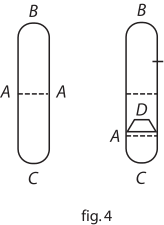
\includegraphics[width=0.3\textwidth]{images/37_3_145v}\\\rule[0cm]{1.7cm}{0cm}\textit{[Fig. 1]}
%                        %\caption{Bildbeschreibung}
%                        \end{wrapfigure}
%                        %@ @ @ Dies ist eine Abstandszeile - fuer den Fall, dass mehrere figures hintereinander kommen, ohne dass dazwischen laengerer Text steht. Dies kann zu einer Fahlermeldung fuehren. @ @ @ \\
                        que le poids\protect\index{Sachverzeichnis}{poids} \textit{D} fait la même chose que feroit l'air \textit{BD} \'{e}gale en consistence \`{a} \edtext{\textit{CD} ou}{\lemma{}\Afootnote{\textit{CD} ou \textit{ erg.} \textit{ L}}} \textit{AC} doublement \edlabel{145vstart}press\'{e}.  Soit l'air $\displaystyle AC=AB=\frac{1}{2}a\rule[-4mm]{0mm}{10mm}$ l'espace $\displaystyle AC=AB=\frac{1}{2}b\rule[-4mm]{0mm}{10mm}$ l'espace $\displaystyle DC=\frac{1}{4}b\rule[-4mm]{0mm}{10mm}$  l'espace $\displaystyle DB=\frac{3}{4}b\rule[-4mm]{0mm}{10mm}$.\edlabel{145vend}\edtext{}{\lemma{press\'{e}.}\xxref{145vstart}{145vend}\Afootnote{ \textit{ (1) }\ Et comme la consistence de \textit{CD} \textit{ (2) }\ L'espace \textit{ (3) }\ Soit [...] $DB=\frac{3}{4}b.$ \textit{ L}}} Donc deux quantitez d'air \'{e}gales \textit{AC} et \textit{AB} occuperont l'une \textit{AB} l'espace \textit{DB} triple de l'espace \textit{DC} qu'occupe l'autre \textit{AC}. Donc pour retenir l'air \textit{AC} dans l'espace \textit{DC} si même le poids\protect\index{Sachverzeichnis}{poids} \textit{D} seroit ost\'{e}, il faut que l'air \textit{AB} en \textit{DB} soit \'{e}galement condens\'{e} avec l'air en \textit{DC} et par consequent il doit estre condens\'{e} trois fois plus qu'il n'est en effect. Donc le poids\protect\index{Sachverzeichnis}{poids} \textit{D} faut autant que deux fois l'air \textit{AB} ou \textit{AC} et par consequent la force du ressort de l'air quoyqu'elle agisse librement, peut estre surmont\'{e}e par un poids\protect\index{Sachverzeichnis}{poids} mediocre, contre ce que j'avois avanc\'{e} au commencement. Supposons \`{a} present que l'air \textit{AB} soit ost\'{e} de \textit{DB} entierement, et l'air \textit{AC} dans l'espace \textit{DC} priv\'{e} d'un tiers de sa quantit\'{e}, ou si vous voulez l'air \textit{AC} laiss\'{e} comme il est dans l'espace \textit{DC} et au lieu de l'air \textit{AB} ost\'{e}, le poids\protect\index{Sachverzeichnis}{poids} \textit{D} augment\'{e} de la moiti\'{e} de ses forces alors le poids\protect\index{Sachverzeichnis}{poids} \textit{D} augment\'{e} contraindra \edtext{ou retiendra}{\lemma{}\Afootnote{ou retiendra \textit{ erg.} \textit{ L}}} l'air en \textit{DC} quoyque la place \textit{DB} soit entierement s'il n'y a point d'autre force que celle du ressort de l'air.\pend